\documentclass[conference]{IEEEtran}
\IEEEoverridecommandlockouts

\usepackage[T1]{fontenc}
\usepackage{amsmath}
\usepackage{graphicx}
\usepackage{booktabs}
\usepackage{tabularx}
\usepackage{array}
\usepackage{xcolor}
\usepackage{microtype}
\usepackage{cite}
\usepackage[hyphens]{url}
\usepackage[hidelinks]{hyperref}
\hypersetup{
  pdftitle={When the Semantic Layer Is Wrong: Do LLM Data Agents Follow or Flag Faulty Business Definitions?},
  pdfauthor={Poorva Barve},
  pdfsubject={Controlled faults in semantic layers for text-to-SQL},
  pdfkeywords={semantic layers, text-to-SQL, robustness, data governance}
}

\newcommand{\id}[1]{\texttt{#1}}
\newcolumntype{L}{>{\raggedright\arraybackslash}X}

\begin{document}

\title{When the Semantic Layer Is Wrong: Do LLM Data Agents Follow or Flag Faulty Business Definitions?%
\thanks{Preprint, November 2026. Not peer reviewed.}}

\author{\IEEEauthorblockN{Poorva Barve}
\IEEEauthorblockA{poorvabarve@gmail.com}}

\maketitle
\pagestyle{plain}
\thispagestyle{plain}

\begin{abstract}
Semantic layers improve text-to-SQL accuracy when their business definitions are correct. We study 24 controlled faults in an Apache Ossie model over TPC-DS, covering formulas, filters, synonyms, fiscal calendars, join keys and value mappings. Each fault has a coherent form, whose documentation agrees with it, and a contradictory form, whose documentation retains the reference definition. In 1,512 single-turn, tool-free trials with three models, a correct layer raised accuracy from 60--71\% to 100\% on this benchmark. Coherent faults were followed in 46--73\% of trials and reduced pooled accuracy relative to no layer by 26 percentage points (95\% CI, 9--43). Contradictory faults were located in 92--100\% of trials but followed in 4--33\%. Some responses raised a concern about the faulted definition and still used it. A generic audit instruction did not reliably reduce following and raised concerns on the correct layer by 17 percentage points. Plausible business conventions may require an independent policy reference to verify. Author annotations of 417 sampled concerns gave agreement with the detection rule of Cohen's $\kappa = 0.89$ for layer concerns and $0.90$ for located faults.
\end{abstract}

\begin{IEEEkeywords}
semantic layer, text-to-SQL, LLM agents, data governance, robustness, silent failure
\end{IEEEkeywords}

\section{Introduction}

LLM data agents increasingly answer business questions through a semantic layer instead of raw tables. Examples include dbt's semantic layer, Snowflake Cortex Analyst semantic models, Cube, and Apache Ossie (incubating)~\cite{ossie}, a vendor-neutral YAML format formerly called the Open Semantic Interchange. A semantic layer defines what ``revenue'', ``fiscal year'' or ``preferred customer'' mean, how tables join, and which words are synonyms.

Several studies report accuracy gains from providing correct semantic context~\cite{rumiantsau2026,kim2026quvi,pillai2026ground,lee2026}. Layers, however, are maintained by hand, and they drift: a metric is redefined, a filter is added for one report, a synonym is attached to the wrong metric, a join key is mistyped. A layer is dangerous when it is wrong \emph{because} it is authoritative. An agent that follows a wrong definition writes a query that runs and returns a plausible number, with no sign that anything is amiss.

We ask what agents do when the layer is wrong:
\begin{itemize}
\item \textbf{RQ1:} How much does a correct layer help?
\item \textbf{RQ2:} Is a wrong element worse than a missing one, or than no layer at all?
\item \textbf{RQ3:} When the layer is wrong, do agents follow it silently? Does it matter whether the fault can be seen by reading the layer?
\item \textbf{RQ4:} Does asking agents to audit the layer help, and what does it cost?
\end{itemize}

To answer them we built a benchmark of 24 business questions over TPC-DS~\cite{tpcds}, each anchored on one element of an Ossie semantic model, and injected a controlled fault of one of six types into that element. Each fault comes in a coherent form, whose documentation agrees with the fault, and a contradictory form, in which only the definition changes. Three models were evaluated across 13 conditions, with five conditions using a 12-question subset: 1,512 trials in all. Every extracted SQL query was executed on Snowflake and its result compared with both the correct answer and the answer the faulty definition produces. Agents also reported structured concerns, which lets us measure \emph{flagging} separately from \emph{following}.

Our contributions are:
\begin{itemize}
\item A fault-injection benchmark for semantic layers: six typed fault operators in coherent and contradictory forms, a gate that guarantees each fault changes the answer on the data, two independently written gold sets, and deterministic grading against Snowflake.
\item Evidence from protocol-specified comparisons that coherent faults are followed far more often than contradictory ones ($+42$ percentage points) and that a wrong element is worse than a missing one ($+33$ percentage points); a coherent wrong element is also worse than no layer at all.
\item The finding that flagging and following are not exclusive: agents often state that a definition looks wrong and then use it.
\item Evidence that a generic audit instruction raises concerns on a correct layer without reliably reducing following, with implications for how products built on semantic layers present agent concerns.
\end{itemize}

\section{Related Work}

\textbf{Semantic layers for LLM analytics.} Rumiantsau and Fokeev~\cite{rumiantsau2026} compare a schema-only prompt with a schema plus a semantic layer in a paired benchmark over three models; they define ``silent hallucination'' but do not measure it. QUVI~\cite{kim2026quvi} routes an agent through a hand-curated layer, GROUND~\cite{pillai2026ground} reduces hallucination with governed definitions, and Lee~\cite{lee2026} treats the layer as the arbiter of business truth while noting that an error in a metric definition can escape both of its checks. All of these studies assume the layer is correct.

\textbf{Wrong evidence in text-to-SQL.} The evidence field of BIRD~\cite{li2023bird} is in effect a small semantic layer. SEED~\cite{yun2025seed} finds incorrect evidence in 105 of 1,534 BIRD development pairs (6.84\%) and shows that correcting it raises accuracy, and Jin et al.~\cite{jin2026annotation} correct the external knowledge in 17 of the 100 examples they re-annotate. These studies analyze naturally occurring annotation errors, and SEED categorizes their types. Our experiment instead injects controlled changes into a full semantic model and scores result matching and reported concerns separately.

\textbf{Robustness benchmarks.} Dr.Spider~\cite{chang2023drspider}, EvoSchema~\cite{zhang2026evoschema} and SAGE~\cite{wang2026sage} perturb the question or the schema, either preserving meaning or changing the database itself; none plants a wrong definition over unchanged data. R-NL2SQL~\cite{tu2026rnl2sql} formalises auxiliary documentation as an input to the task but does not perturb it.

\textbf{Silent failure.} DiscRun-Bench~\cite{chen2026discrun} scores data correctness and caveats separately for agents doing data preparation. Mismatches between documentation and data format almost never surfaced: they were missed in 18 of 19 and 18 of 18 runs.

\textbf{Knowledge conflicts and documentation errors.} LLMs readily follow coherent, convincing context that conflicts with what they know, and they often notice a conflict without locating it~\cite{xu2024conflicts}. In code, incorrect docstrings hurt models' code understanding more than missing ones~\cite{macke2024docs}, the closest precedent for ``wrong is worse than missing''.

Our study complements this work by measuring both following and flagging after controlled semantic-layer changes, and by contrasting coherent with contradictory documentation. This is a targeted comparison with related work; it does not establish that the underlying knowledge-conflict mechanism is new.

\section{Benchmark and Method}

The protocol, hypotheses, outcome definitions and analysis plan were fixed before the main run. Changes made after the pilot are documented in a post-pilot amendment (Section~\ref{sec:pilot}).

\subsection{Data and Execution}

TPC-DS at scale factor~1 was generated deterministically with DuckDB's \id{dsdgen}~\cite{duckdb} and loaded into Snowflake; all 24 tables were verified column by column. Agents write Snowflake SQL. Each query is first checked with \id{sqlglot}~\cite{sqlglot} to be a single \id{SELECT}, then executed in an isolated container by a read-only key-pair user with a 120\,s statement limit.

\subsection{Semantic Layer}

The base layer is the Ossie TPC-DS example at revision \id{2fd19c7a}~\cite{ossie}, with logged edits: sources were retargeted; three metric descriptions were made explicit about their formulas; fields, metrics and synonyms were added for the fault operators; two conflicting synonyms were removed; and a fan-out error in the example's \id{store\_productivity} metric was fixed, which divided by a sum of employee counts taken over joined sales rows. All 75 layer files used in the study validate against Ossie's JSON schema.

\subsection{Questions and Faults}

There are 24 business questions, four for each of six fault operators (Table~\ref{tab:operators-def}). Each question is anchored on one business definition; its fault changes the corresponding element or, for fiscal definitions, the two related fields. The fault has two forms:
\begin{itemize}
\item \textbf{F1, coherent:} the element's description is edited to agree with the fault, so the layer is internally consistent.
\item \textbf{F2, contradictory:} only the expression, mapping or join changes, so the definition disagrees with its own documentation.
\end{itemize}
Every (question, fault) pair passes a discriminability gate: on the data, the faulty definition gives a different answer from the reference definition. Here, ``faulty means a departure from the benchmark reference. A coherent change to a business convention, such as the fiscal-year start, may be impossible to distinguish from a legitimate policy change using the supplied context alone. These trials measure reliance on the supplied definition; they do not assume the agent can recover an undisclosed policy.

Gold queries were written twice. The second set was written by a separate model that saw only the questions, the layer and the DDL. The two sets agree on all 24 questions, and DuckDB and Snowflake return identical results.

\begin{table}[t]
\caption{Fault operators, with one example each}
\label{tab:operators-def}
\centering
\footnotesize
\begin{tabularx}{\columnwidth}{@{}p{1.75cm}L@{}}
\toprule
Operator & Example fault \\
\midrule
Formula drift & \id{total\_sales} sums \id{ss\_net\_paid} instead of \id{ss\_ext\_sales\_price} \\
Hidden filter & \id{distinct\_customers} counts only customers on profitable lines (\id{ss\_net\_profit > 0}) \\
Synonym & ``department'' is mapped to \id{i\_class} instead of \id{i\_category} \\
Fiscal definition & \id{fiscal\_year} and \id{fiscal\_quarter} start the fiscal year in July instead of February \\
Relationship key & sales join customers on \id{ss\_addr\_sk} $=$ \id{c\_customer\_sk} \\
Value mapping & \id{store\_size\_class} calls a store large from 240 employees instead of 270 \\
\bottomrule
\end{tabularx}
\end{table}

\subsection{Arms}

Table~\ref{tab:arms} lists the thirteen arms. The audit instruction reads: ``Before answering, check the semantic model against the table definitions and the question, and report any problem you find in `concerns'.'' The named-suspect instruction instead asks the agent to check ``the semantic model's definition of'' the anchored element, or of the synonym for synonym faults.

\begin{table}[t]
\caption{Arms. N, C1a and C1b use a 12-question subset}
\label{tab:arms}
\centering
\footnotesize
\begin{tabularx}{\columnwidth}{@{}lLr@{}}
\toprule
Arm & Shown to the agent & Questions \\
\midrule
C0 & Table definitions (DDL) only & 24 \\
C1 & DDL and the correct layer & 24 \\
E & Correct layer with the anchored element removed & 24 \\
F1, F2 & Faulty layer (coherent, contradictory) & 24 \\
C1+A, F1+A, F2+A & As C1, F1, F2, plus the generic audit instruction & 24 \\
C1+N, F1+N, F2+N & As C1, F1, F2, plus an instruction naming the anchored element as suspect & 12 \\
C1a, C1b & Correct layer without metrics; without descriptions and \id{ai\_context} & 12 \\
\bottomrule
\end{tabularx}
\end{table}

\subsection{Agents}

The models were Claude Opus 5.5 (high effort), GPT-6.1 Sol (high reasoning) and Claude Haiku 5.5 (medium effort), with two repetitions per question and arm: 1,512 trials in total. Each trial is a single turn with no tools, so the agent cannot run queries. The system prompt is identical across arms. It says that the organization maintains a semantic model, and it tells the agent neither to trust the model nor to verify it. The agent answers with one JSON object holding \id{sql}, \id{assumptions}, a list of structured \id{concerns} (each with a target of \emph{layer}, \emph{question}, \emph{data} or \emph{other}, an object identifier and a short text) and a \id{confidence}.

\subsection{Outcomes}

All outcomes are computed by deterministic code frozen before dispatch. Each answer is classed as \emph{correct} (its result equals the gold result, including equivalent forms that the layer's descriptions license), \emph{followed} (its result equals the faulty definition's result), \emph{other wrong}, or \emph{no usable answer}. \textbf{D1} is a layer-targeted concern that names something in the layer shown. \textbf{D2} is a D1 concern that names the faulted element, an identifier the fault changed, or the moved synonym. A \textbf{silent failure} is a followed answer with no D1 concern. On the correct layer, D1 measures concerns raised about a layer with no planted fault.

\subsection{Human Check of the Detection Rule}
\label{sec:audit}

The author labelled a 20\% sample of concerns, stratified by arm: 417 concerns from 376 trials, supplying two judgments and a note for every concern. The complete annotations are included with the sample. Labelling was blind to the rule's output and to the model. Each concern received two labels: whether it is about the semantic layer and, when a fault was planted, whether it identifies that fault. Table~\ref{tab:audit} compares these labels with the rule; intervals come from a bootstrap over trials (10,000 resamples). For D1, the rule agreed on 94.5\% of concerns, $\kappa = 0.89$ [0.85, 0.93]~\cite{cohen1960kappa}; its precision was 0.995 [0.98, 1.0] and its recall 0.90 [0.86, 0.94]. For D2, on the 219 concerns from fault arms, agreement was 95.4\% ($\kappa = 0.90$ [0.84, 0.96]), with precision and recall both 0.96 and five errors in each direction.

\begin{table}[t]
\caption{Detection rule against the author's labels}
\label{tab:audit}
\centering
\footnotesize
\setlength{\tabcolsep}{3.5pt}
\begin{tabular}{@{}lrrlrr@{}}
\toprule
Label & $n$ & Agree & $\kappa$ [95\% CI] & Prec. & Recall \\
\midrule
D1 (about the layer) & 417 & 0.945 & 0.89 [0.85, 0.93] & 0.995 & 0.898 \\
D2 (names the fault) & 219 & 0.954 & 0.90 [0.84, 0.96] & 0.962 & 0.962 \\
D2 without Q13--Q16 & 185 & 0.951 & 0.90 [0.83, 0.96] & 0.964 & 0.955 \\
\bottomrule

\end{tabular}
\end{table}

\subsection{Analysis}

The four protocol-specified comparisons are paired by question:
\begin{itemize}
\item \textbf{H1:} following is higher on F1 than on F2;
\item \textbf{H2:} correctness is higher on E than on F1;
\item \textbf{H3a:} D2 on F2 is higher with the audit instruction;
\item \textbf{H3b:} D1 on the correct layer is higher with the audit instruction.
\end{itemize}
Intervals are 95\% cluster-bootstrap intervals over questions (10,000 resamples)~\cite{field2007bootstrap}, with a sensitivity analysis that resamples the six fault operators instead, and a logistic generalized estimating equation (GEE) check~\cite{liang1986gee}. GEE replaces the mixed-effects logistic check named in the draft protocol; the paired bootstrap remains the primary analysis. When an arm has a constant outcome, the logistic check is omitted because of separation. Comparisons added after the pilot are labelled exploratory (X1--X5).

\subsection{Pilot and Amendment}
\label{sec:pilot}

A 180-trial pilot (\$4.02) found two benchmark defects, both fixed before the main run. First, the TPC-DS source flag \id{d\_weekend = \textquotesingle Y\textquotesingle} marks Fridays and Saturdays, so the base layer's weekend definition was itself wrong; question Q22 was redesigned. Second, TPC-DS injects NULLs independently into derived columns, so formulas computed from component columns are now accepted as equivalent. The main run cost \$36.41 for 1,512 trials, all of which completed. Total model spend for the study was \$40.44.

\section{Results}

Table~\ref{tab:outcomes} gives the main outcomes by model, Fig.~\ref{fig:outcomes} shows every arm, and Table~\ref{tab:comparisons} lists all paired comparisons.

\begin{table}[t]
\caption{Correct and followed rates by model (48 trials per cell)}
\label{tab:outcomes}
\centering
\footnotesize
\setlength{\tabcolsep}{3.5pt}
\begin{tabular}{@{}lrrrrrrr@{}}
\toprule
& \multicolumn{3}{c}{Correct} & \multicolumn{2}{c}{F1 (coherent)} & \multicolumn{2}{c}{F2 (contradict.)} \\
\cmidrule(lr){2-4}\cmidrule(lr){5-6}\cmidrule(l){7-8}
Model & C0 & C1 & E & Correct & Follow. & Correct & Follow. \\
\midrule
Opus & 71\% & 100\% & 79\% & 52\% & 46\% & 96\% & 4\% \\
Sol & 62\% & 100\% & 69\% & 23\% & 73\% & 67\% & 33\% \\
Haiku & 60\% & 100\% & 67\% & 42\% & 56\% & 88\% & 12\% \\
\bottomrule

\end{tabular}
\end{table}

\begin{figure*}[t]
\centering
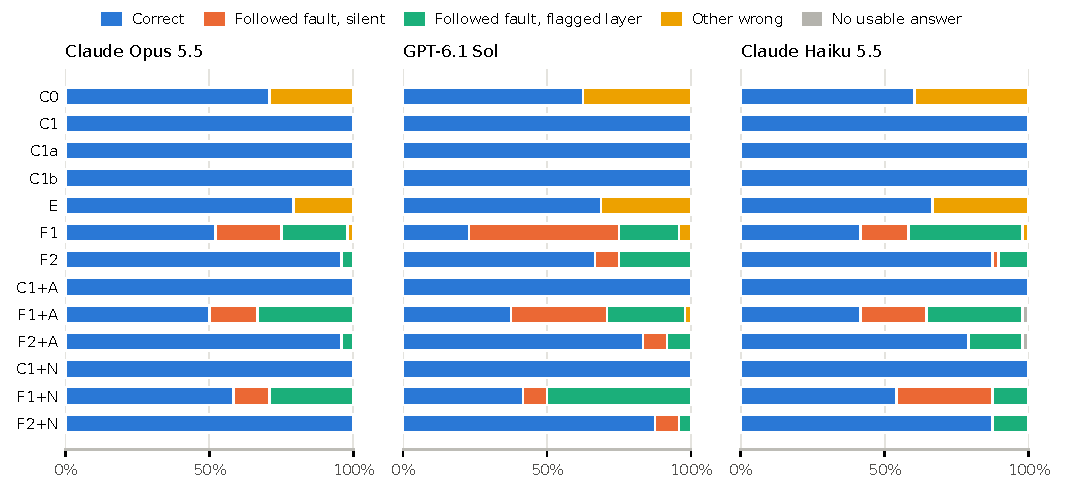
\includegraphics[width=\textwidth]{figures/outcomes.pdf}
\caption{Outcome of every trial, by model and arm. ``Followed fault, flagged layer'' means the result equals the faulty definition's result and the same response raised a layer concern (D1). In arms without a fault, a result that happens to equal the faulty result is counted as other wrong. The N, C1a and C1b arms have 24 trials per model; all other arms have 48.}
\label{fig:outcomes}
\end{figure*}

\begin{table*}[t]
\caption{Paired comparisons in percentage points, clustered by question. H: protocol-specified; X: exploratory; RQ2: named in the protocol without a specified direction. GEE is omitted for X4 because C1 is constant}
\label{tab:comparisons}
\centering
\footnotesize
\begin{tabular}{@{}lllrlll@{}}
\toprule
ID & Outcome & Contrast & Estimate & 95\% CI (questions) & 95\% CI (operators) & GEE $p$ \\
\midrule
H1 & Followed & F1 $-$ F2 & $+42$ & [+27, +56] & [+18, +69] & $<0.001$ \\
H2 & Correct & E $-$ F1 & $+33$ & [+18, +48] & [+11, +54] & $<0.001$ \\
H3a & D2 & F2+A $-$ F2 & $-1$ & [$-$4, +1] & [$-$3, +1] & 0.346 \\
H3b & D1 & C1+A $-$ C1 & $+17$ & [+5, +29] & [+4, +29] & 0.011 \\
\midrule
X1 & Followed & F2 $-$ F2+A & $+3$ & [$-$1, +9] & [$-$3, +10] & 0.252 \\
X2 & Followed & F1 $-$ F1+A & $+3$ & [$-$3, +8] & [0, +6] & 0.338 \\
X3 & Silent & F1 $-$ F1+A & $+6$ & [$-$3, +15] & [$-$4, +16] & 0.188 \\
X4 & Correct & C1 $-$ C0 & $+35$ & [+19, +53] & [+8, +67] & -- \\
X5 & Correct & E $-$ C0 & $+7$ & [+1, +15] & [+1, +16] & 0.067 \\
\midrule
RQ2 & Correct & C0 $-$ F1 & $+26$ & [+9, +43] & -- & -- \\
RQ2 & Correct & C0 $-$ F2 & $-19$ & [$-$40, +2] & -- & -- \\
\bottomrule

\end{tabular}
\end{table*}

\subsection{RQ1: A Correct Layer Helps}

Without a layer, agents answered 60--71\% of questions correctly; with the correct layer, every model answered every question correctly (Table~\ref{tab:outcomes}). The pooled difference is $+35$ percentage points [+19, +53] (X4). Without a layer, agents miss business definitions they cannot infer from the schema: the fiscal calendar, which categories count as apparel, the store-size threshold, what ``preferred'' means. Removing only the anchored element (E) keeps part of the layer's benefit for the rest of the question: E $-$ C0 $= +7$ [+1, +15] (X5). On the 12-question subset, removing metrics (C1a) or descriptions and \id{ai\_context} (C1b) left all 72 responses correct in each arm. The remaining context was sufficient on that subset; these ceiling results do not establish which construct carries the gain on other tasks.

\subsection{RQ2: A Wrong Element Is Worse than a Missing One, and Worse than None}

With the anchored element removed, accuracy was 67--79\%; with a coherent fault in it, 23--52\%. H2 is supported: E $-$ F1 $= +33$ percentage points [+18, +48], robust to operator clusters [+11, +54] and to the GEE check ($p < 0.001$). A coherent wrong element is also worse than no layer at all: C0 $-$ F1 $= +26$ percentage points [+9, +43], that is $+19$ for Opus and Haiku and $+40$ for Sol. This comparison is named in the protocol's RQ2 without a direction specified in advance. We found no clear evidence that contradictory faults reduced accuracy relative to no layer: C0 $-$ F2 $= -19$ [$-40$, +2].

\subsection{RQ3: Coherent Faults Are Followed, Sometimes Despite a Located Concern}

Coherent faults were followed in 46\% (Opus), 73\% (Sol) and 56\% (Haiku) of trials, and contradictory faults in 4\%, 33\% and 12\%. H1 is supported: F1 $-$ F2 $= +42$ percentage points [+27, +56], consistent across models ($+42$, $+40$, $+44$ for Opus, Sol and Haiku) and robust to operator clusters [+18, +69] and to the GEE check ($p < 0.001$).

Silent failure, that is following with no layer concern, occurred in 23\% of F1 trials for Opus, 52\% for Sol and 17\% for Haiku (Table~\ref{tab:detection}). A general layer concern (D1) accompanied 19 of Haiku's 27 F1 follows, 11 of Opus's 22 and 10 of Sol's 35. A located concern (D2) accompanied 14/27, 9/22 and 10/35, respectively. The difference matters: a concern about an unrelated metric does not establish that the followed fault was noticed. On F2, Sol raised a located concern in 12 of its 16 follows. For example, Opus's Q06 F1 response (repetition 1) described the planted NULL-store filter in \id{total\_quantity} but still applied that filter in its query.

\begin{table}[t]
\caption{Detection on faulty and correct layers. Silent: share of F1 trials that followed the fault with no layer concern. Located: F1 follows that raised a D2 concern, out of all F1 follows}
\label{tab:detection}
\centering
\footnotesize
\setlength{\tabcolsep}{3pt}
\begin{tabular}{@{}lrrrrrrr@{}}
\toprule
& \multicolumn{4}{c}{F1 (coherent)} & F2 & C1 & C1+A \\
\cmidrule(lr){2-5}\cmidrule(lr){6-6}\cmidrule(lr){7-7}\cmidrule(l){8-8}
Model & D1 & D2 & Silent & Located & D2 & D1 & D1 \\
\midrule
Opus & 77\% & 73\% & 23\% & 9/22 & 100\% & 23\% & 52\% \\
Sol & 48\% & 48\% & 52\% & 10/35 & 92\% & 2\% & 6\% \\
Haiku & 83\% & 73\% & 17\% & 14/27 & 98\% & 35\% & 52\% \\
\bottomrule

\end{tabular}
\end{table}

Following depends strongly on the operator (Table~\ref{tab:operators}). No coherent wrong join key was followed, while every coherent fiscal-year fault was followed, two thirds of them silently. In these tasks, schema-visible conflicts coincided with lower following: joining \id{ss\_addr\_sk} to \id{c\_customer\_sk} conflicts with the column names' apparent meanings. Following was higher for plausible business conventions: a July fiscal start, a 240-employee threshold, which categories count as apparel.

\begin{table}[t]
\caption{Following and detection by fault operator, all models pooled (24 trials per operator and arm)}
\label{tab:operators}
\centering
\footnotesize
\setlength{\tabcolsep}{3.5pt}
\begin{tabular}{@{}lrrrrr@{}}
\toprule
& \multicolumn{2}{c}{F1} & \multicolumn{2}{c}{F2} & F1+A \\
\cmidrule(lr){2-3}\cmidrule(lr){4-5}\cmidrule(l){6-6}
Operator & Followed & Silent & Followed & D2 & Followed \\
\midrule
Formula drift & 54\% & 17\% & 17\% & 100\% & 54\% \\
Hidden filter & 71\% & 29\% & 12\% & 100\% & 62\% \\
Synonym & 50\% & 17\% & 33\% & 92\% & 42\% \\
Fiscal definition & 100\% & 67\% & 0\% & 100\% & 100\% \\
Relationship key & 0\% & 0\% & 0\% & 100\% & 0\% \\
Value mapping & 75\% & 54\% & 38\% & 88\% & 75\% \\
\bottomrule

\end{tabular}
\end{table}

\subsection{RQ4: An Audit Instruction Raises Concerns Without a Clear Reduction in Following}

H3a is not supported: located detection on F2 is already at ceiling (92--100\%), and the audit instruction changes it by $-1$ point [$-4$, +1]. H3b is supported: the audit raises concerns on the correct layer by $+17$ percentage points [+5, +29] (operator clusters [+4, +29]; GEE $p = 0.011$), from 23\% to 52\% for Opus, 2\% to 6\% for Sol and 35\% to 52\% for Haiku.

In exploratory comparisons, the audit barely reduced following: by 3 percentage points [$-1$, +9] on contradictory faults (X1), where Sol gained most ($+17$) and Haiku did slightly worse ($-6$), and by 3 percentage points [$-3$, +8] on coherent faults (X2). Naming the suspect element (F1+N) raised located detection of coherent faults to 88\% for Opus, 92\% for Sol and 62\% for Haiku, yet agents still followed the fault in 42--58\% of those trials.

Concerns on the reference layer are not all false alarms. On C1, they frequently targeted \id{total\_profit}: its description uses component arithmetic while its expression uses a derived column. Other concerns addressed definitional choices in customer lifetime value and average ticket value, or the example's ``manufacturer'' synonym for \id{i\_brand}. The author labels establish whether a concern is about the layer, rather than whether it is justified; separating substantive concerns from noise remains open.

\section{Discussion}

\textbf{Coherent faults received less resistance.} Models located documentation and schema conflicts more often than coherent departures from the reference. A plausible policy change may leave no visible conflict. Such cases motivate independent policy references rather than assuming the model can recover an undisclosed convention.

\textbf{Concerns require a response policy.} Some responses raise a located concern and still use the associated definition. A pipeline that displays the number but hides the concern can therefore conceal a detected problem. Products should surface relevant concerns or consider abstaining when a concern names an element used by the query.

\textbf{Prompting for skepticism.} The generic audit raised concerns without a clear reduction in following. Verifying a coherent convention can require an approved policy, ledger reconciliation or independent tests; data profiles alone may not establish business intent. Follow-up work could test tool-using agents and semantic layers carrying assertions, such as reconciliation of a sales metric with a finance ledger.

\textbf{Model differences.} GPT-6.1 Sol had the highest observed following and silent-following rates. Claude Opus 5.5 had the lowest following rate, while Claude Haiku 5.5 often raised concerns alongside followed answers. These comparisons describe the tested prompts and tasks rather than general model traits.

\textbf{Implications for Ossie.} Building the benchmark surfaced two problems in the official example: a metric whose plain-SQL reading double-counts under joins, and a misleading synonym (``manufacturer'' for brand). A linter that checks descriptions against expressions, and flags model-scoped metrics with ambiguous join paths, could help identify such inconsistencies; we did not implement or evaluate that linter.

\section{Threats to Validity}
\label{sec:threats}

\textbf{Scale.} There are 24 questions on one public schema, and models may know TPC-DS conventions. The intervals are wide and question-level, and the 12-question subset arms are smaller still.

\textbf{Injected faults.} The faults are injected, not natural, and their plausibility is argued rather than measured. The author wrote the layer additions, the faults and the first gold set; the second gold set was written by a model. The Q22 redesign and the equivalence grading changed after the pilot and before the main run, and both are documented.

\textbf{Base-layer imperfections.} Some descriptions in our base layer do not match their expressions exactly (for example \id{total\_profit}), which raises concerns on the correct layer. All base-layer edits are logged.

\textbf{Detection is rule-based and conservative.} Against the author's labels, the rule almost never over-counts D1 (precision 0.995). It misses about one layer concern in ten, and two kinds account for almost all the misses: concerns that the layer \emph{lacks} a definition, which name no layer identifier, and layer concerns filed under the question or the data. Misses concentrate in arm E, where D1 agreement is 78\%, so D1 rates can be underestimated, especially for E, and missed concerns can inflate measured silent failure. D2 errors are balanced. Free-text concerns that do not use the structured \id{object} field are not counted.

\textbf{Limits of the human check.} It used one rater. The original sample display described only \id{fiscal\_year} for Q13--Q16, although the fault also changed \id{fiscal\_quarter}. The author notes explicitly consider both fields. As a sensitivity analysis, excluding these 34 concerns leaves D2 agreement unchanged at $\kappa = 0.90$ (Table~\ref{tab:audit}).

\textbf{Single turn, no tools.} The results do not describe agents that can query the data.

\textbf{Literature.} The related-work comparison is targeted rather than systematic, so relevant studies may be missing.

\textbf{Statistics.} The GEE check is omitted for X4 because every model scores 100\% on C1. Operator-cluster intervals rely on only six clusters and should be interpreted cautiously.

\section{Conclusion}

On this benchmark, a correct semantic layer raised accuracy from 60--71\% to 100\%, while coherent faults were followed in 58\% of trials and left agents worse off than no layer. Some responses used a definition despite a located concern, and a generic audit instruction mostly added concerns. Independent policy evidence, relevant-concern handling and checkable assertions are promising directions for semantic-layer reliability.

\section*{Data and Code Availability}

The repository, \url{https://github.com/barveP/semantic-layer-trust-paper}, is currently private. It contains benchmark inputs, prompts, frozen plans, graded trials, analysis code and all 417 author annotations with notes. The documented build regenerates the result and audit tables. Historical freeze records and later reporting changes are distinguished in the README. Full experiment reruns additionally require Snowflake, generated TPC-DS data and an external dispatcher not distributed here. Credentials and unparsed responses are excluded.

\bibliographystyle{IEEEtran}
\bibliography{references}

\end{document}
